\documentclass[handout]{beamer}
\usepackage[utf8]{inputenc}
\usepackage{graphics}
\mode<presentation> {
\usetheme{unc}}
\setbeamertemplate{navigation symbols}{} % To remove the navigation symbols from the bottom of all slides uncomment this line

\usepackage{graphicx} % Allows including images
\usepackage{booktabs} % Allows the use of \toprule, \midrule and \bottomrule in tables


\usepackage{hyperref}
\hypersetup{linkcolor=blue,colorlinks=true}


% Remove symbols
\beamertemplatenavigationsymbolsempty


%\usetheme{default}

\usefonttheme{serif}

%----------------------------------------------------------------------------------------
%	TITLE PAGE
%----------------------------------------------------------------------------------------


\title[Introduction]{\LARGE{POLI 150: International Relations and Global Politics}}
\author[POLI 150]{Steven Saroka}
\institute{POLI 150}
\date{11 January 2024}


\begin{document}

\begin{frame}
\titlepage % Print the title page as the first slide
\end{frame}


%\begin{frame}
%\frametitle{Overview} % Table of contents slide, comment this block out to remove it
%\tableofcontents % Throughout your presentation, if you choose to use \section{} and \subsection{} commands, these will automatically be printed on this slide as an overview of your presentation
%\end{frame}

%----------------------------------------------------------------------------------------
%	PRESENTATION SLIDES
%----------------------------------------------------------------------------------------



\begin{frame} 
	\frametitle{\LARGE{Today's Class}}
	\begin{itemize}
		\Large{
			\item Introductions
			\\~\\ 
			\item Syllabus and Expectations
			\\~\\
			\item Why Study IR? 
			}
	\end{itemize}
\end{frame}

\begin{frame} 
	\frametitle{\LARGE{Introduction}}
	\begin{itemize}
		\item Instructor: Steven Saroka
		\\~\\
		\item Email: ssaroka@ad.unc.edu
		\\~\\
		\item Office Hours: by appointment via Zoom on Mondays and Wednesdays from 3-4:30 PM. \href{https://www.signupgenius.com/go/10C0F48AFAD29A6FDCF8-47020746-poli\#/}{Sign up link.}
	\end{itemize}
\end{frame}

%\begin{frame} 
%\frametitle{\LARGE{Your Turn}}
%\begin{enumerate}
%	\large{
%		\item Name
%		\\~\\ 
%		\item Preferred pronouns
%		\\~\\
%		\item Major and year
%		\\~\\
%		\item Where you're from
%		\\~\\
%		\item Something new you've picked up this past year: a hobby, show, novel or author, interest, work
%	}
% \end{enumerate}
% \end{frame}

\begin{frame}{\LARGE Course Structure: Meeting and Readings}
	\begin{itemize}
		\item Meeting: Tuesdays and Thursdays 2-3:15 PM, Murphey Hall 104.
		\item Most classes have readings assigned, listed in syllabus. These are to be completed before the lectures for which they are assigned.
		\item Textbook: Frieden, Lake, and Schultz's \textit{World Politics: Interests, Interactions, Institutions} 4th edition.
		\begin{itemize}
			\item \textbf{Not 5th edition}
	%		\item \href{https://www.google.com/search?client=firefox-b-1-d&q=world+politics+interests+interactions+institutions+4th+edition+pdf}{Rent, buy used, or find on your own...}    	
		\end{itemize}
		\item All other readings are posted on Canvas under ``Files" then ``Readings"
	\end{itemize}
\end{frame}

\begin{frame}{\LARGE Course Structure: Assignments}
	Your final grade is composed of: 
	\begin{itemize}
		\item 2 midterms worth 15\% each.
		\begin{itemize}
			\item 15-20 multiple choice; open note and book; non-cumulative.
		\end{itemize}
		\item 10 short reflection papers worth 5\% each.
		\begin{itemize}
			\item One page, single- or double-spaced.
			\item Turn in 10 out of 13 prompts; posted on Canvas.
		\end{itemize}
		\item Final: 20\%
		\begin{itemize}
			\item 15-20 multiple choice; open note and book; cumulative.
		\end{itemize}
	\end{itemize}
\end{frame}


\begin{frame}{\LARGE Assignment Important Dates}
	\begin{itemize}
		\item Reflection papers: generally due 1 week after their associated topic at 11:59 PM. Submit on Canvas.
		\item Exams: Mar. 7 and Apr. 18. Final available from Apr. 30 to May 3 at 11:59 PM. 
	\end{itemize}
\end{frame}

\begin{frame} 
	\frametitle{\LARGE{Expectations for Papers}}
	\begin{itemize}
		\item Maximum length of one page.
		\item Submitted as Word document.
		\item Double- or single-spaced, 12-point font.
		\item Citations not required unless using an outside source (non-textbook, non-lecture).
		\item Use of AI must follow policy in syllabus.
	\end{itemize}
\end{frame}

\begin{frame}{\LARGE General Expectations}
	\begin{itemize}
		\item Contacting me: email or office hours
		\\~\\
		\item Classroom civility
		\\~\\
		\item Attendance and excused absences
		\\~\\
		\item ARS accommodations: please contact me privately via email
	\end{itemize}
\end{frame}

\begin{frame}{\LARGE What is International Relations (IR)?}
    \begin{itemize}
        \item Understanding the interactions between political units in world politics 
        \item What is a ``political unit" anyway? \pause
        \begin{itemize}
        \item Example from American politics: Congress, Presidency, Supreme Court
   		\end{itemize}
        \item Abstract up to the level of international relations, and it's no longer so simple...
    \end{itemize}
\end{frame}

\begin{frame}
\frametitle{\LARGE{What is IR?}}
\begin{itemize}
	\item IR has traditionally focused on the most obvious political units in world politics: countries (``states" in most IR literature).
	\item States are entities that have:
	\begin{itemize}
		\item A central authority \pause
		\item with the ability to make laws, rules, and decisions \pause
		\item and enforce them via a monopoly on the use of violence \pause
		\item within a specified territory \pause
		\item recognized as sovereign by other states \pause
	\end{itemize}
	\item IR has traditionally examined relationships between states: wars, alliances, trade, commerce, cooperation on global issues (environment, human rights), etc.
\end{itemize}
\end{frame}

\begin{frame}
\frametitle{\LARGE{What is IR?}}

Today the field of IR involves the relationships between states but also the study of many more interactions, including:
\begin{itemize}
	\item States and rebel groups \pause
	\item States and international institutions like the UN \pause
	\item Multinational corporations and the states they operate in \pause
	\item Terrorist groups and states \pause
	\item Interactions of these actors absent states \pause
\end{itemize}
Still: States remain the foundational actor in most analysis.
\end{frame}

\begin{frame}{\LARGE Some class topics} %http://www.systemicpeace.org/conflicttrends.html#fig3
\centering
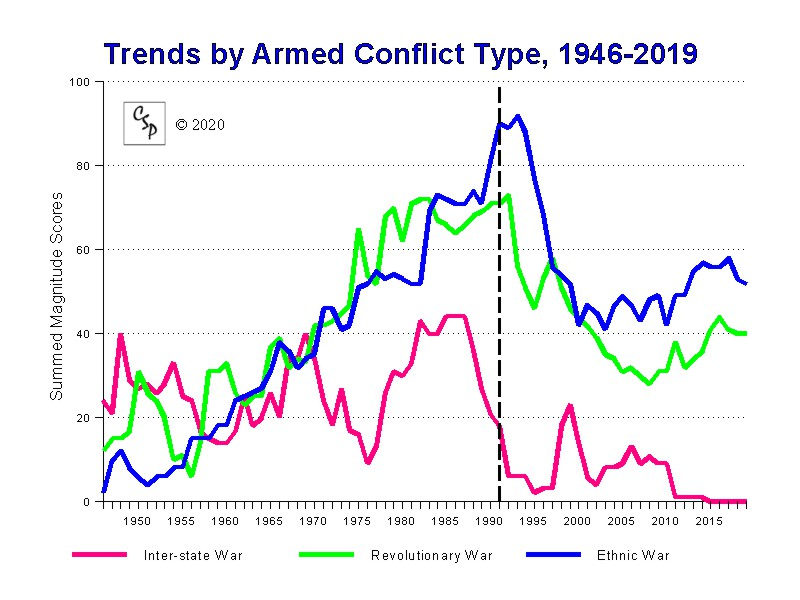
\includegraphics[width=\textwidth,height=0.9\textheight,keepaspectratio]{wartyp19.jpg}
\end{frame}

\begin{frame}{\LARGE Some class topics} %https://www.prio.org/Projects/Extensions/ConflictTrends/Graphs/?xitem=1631&handler=Project
	\centering
	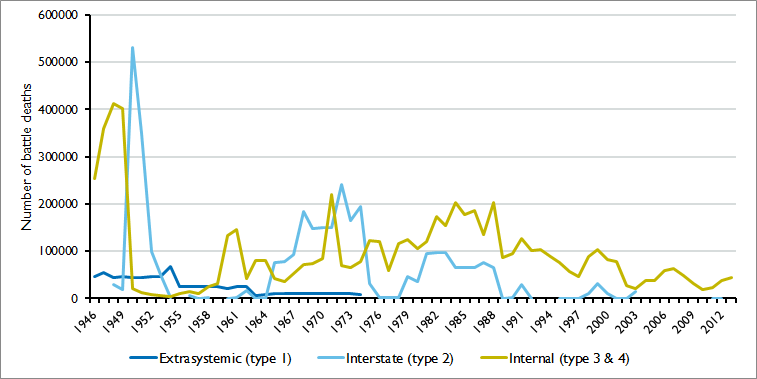
\includegraphics[width=\textwidth]{battledeathnumbers.png}
\end{frame}

\begin{frame}{\LARGE Some class topics}  %https://www.prio.org/utility/DownloadFile.ashx?id=1373&type=publicationfile
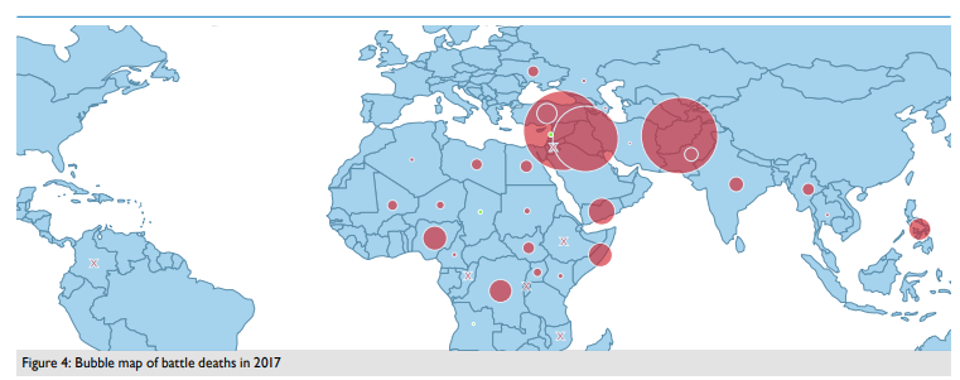
\includegraphics[width=\textwidth]{battle deaths.png}
\end{frame}

\begin{frame}{\LARGE Some class topics}
\centering
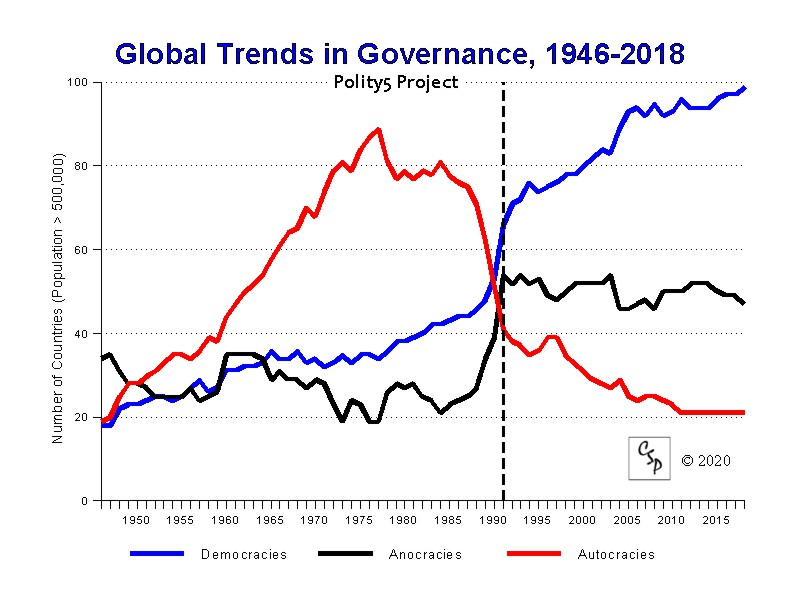
\includegraphics[width=\textwidth,height=0.8\textheight,keepaspectratio]{Global trends governance.jpg}
\end{frame}

\begin{frame}{\LARGE Some class topics}
\centering
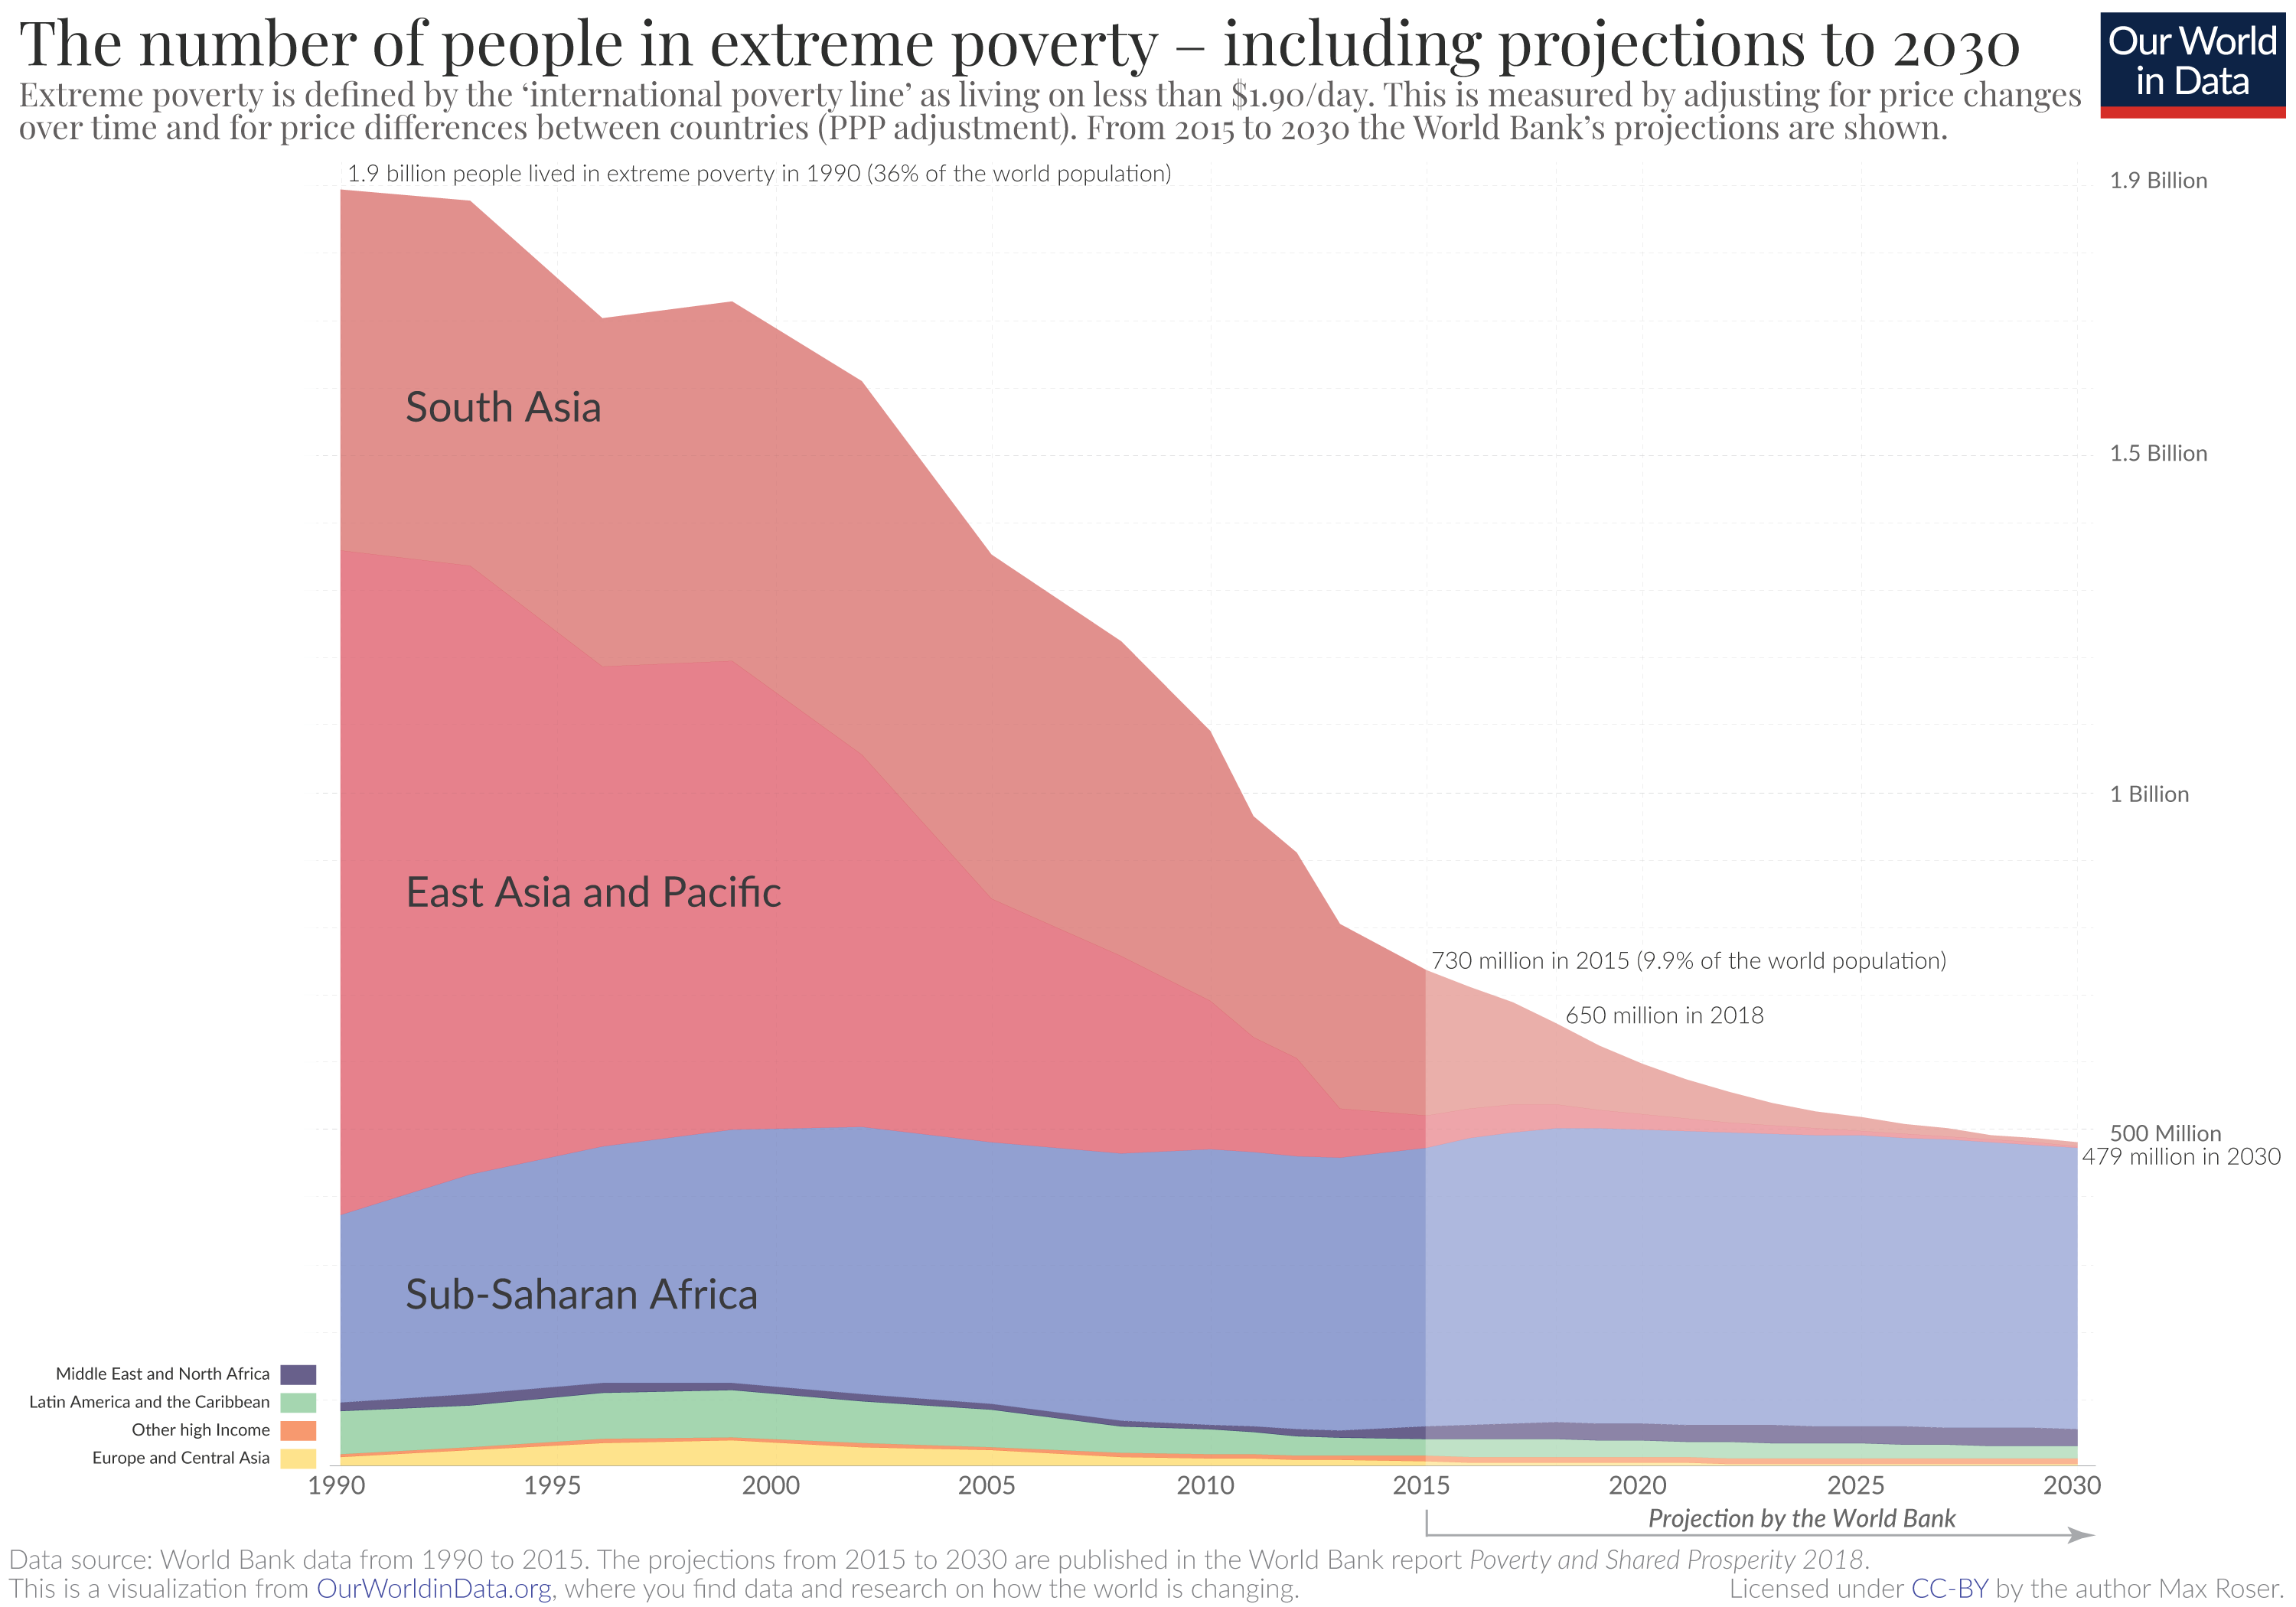
\includegraphics[width=\textwidth,height=0.8\textheight,keepaspectratio]{Extreme-Poverty-projection-by-the-World-Bank-to-2030.png}
\end{frame}

\begin{frame}{\LARGE Some class topics} %pulled from Layna's intro, but no source there
	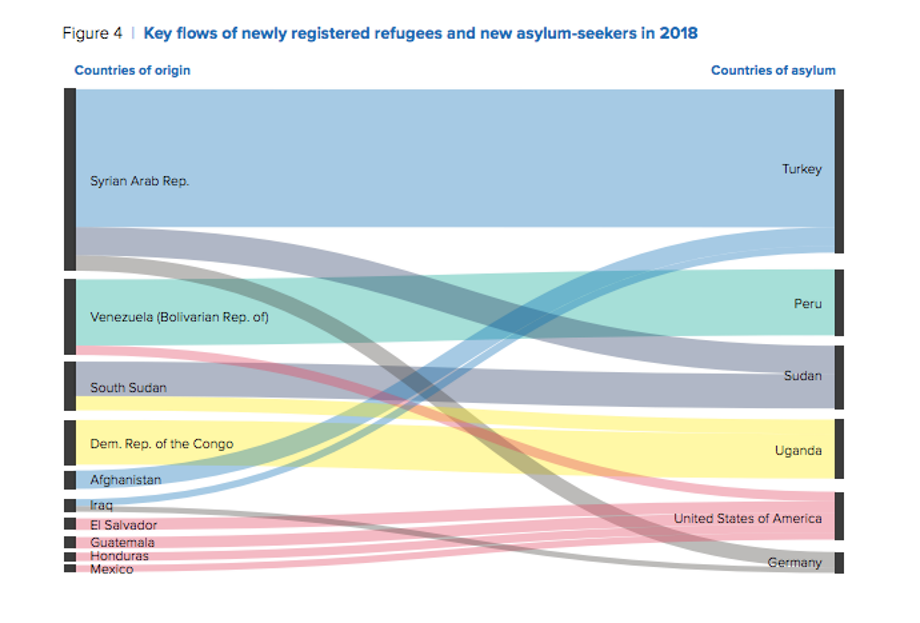
\includegraphics[width=\textwidth]{refugee flows.png}
\end{frame}

\begin{frame}{\LARGE Some class topics}
\centering
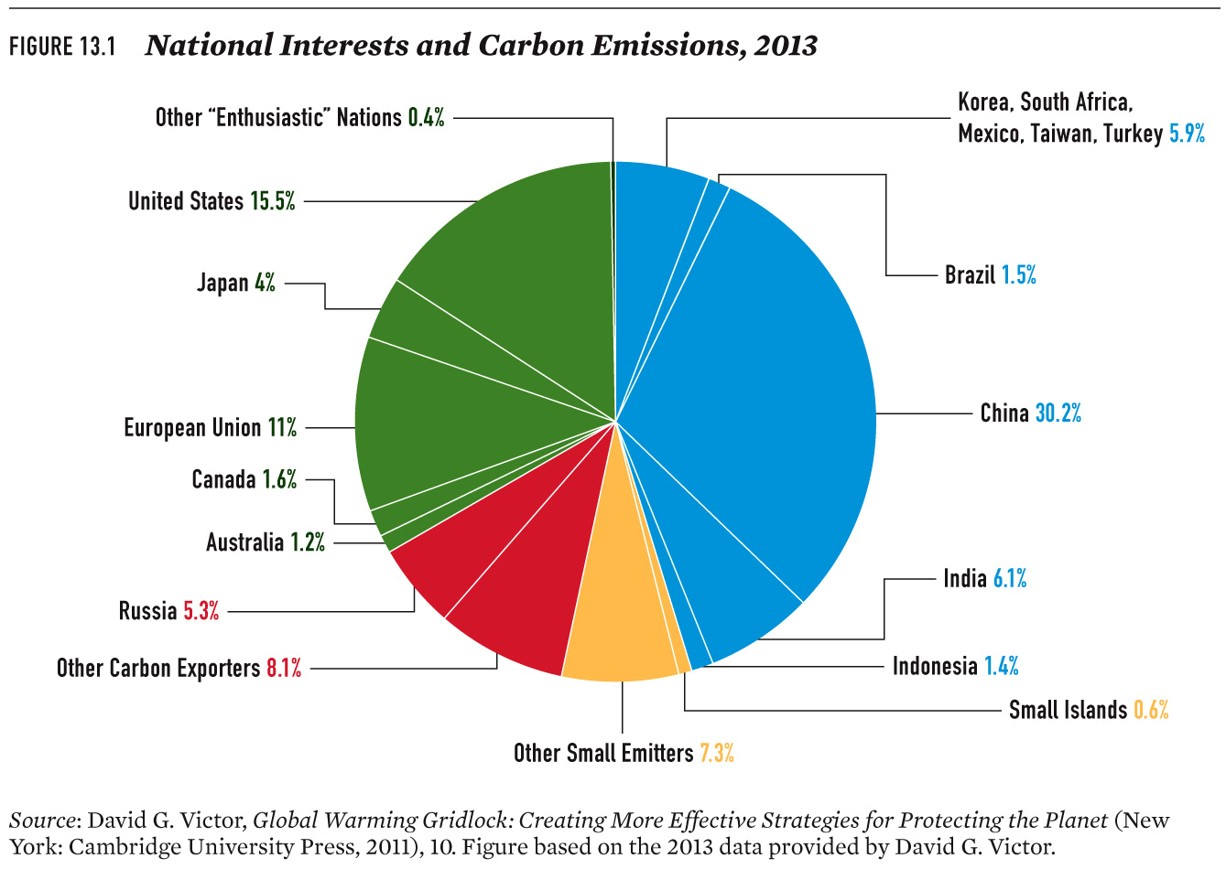
\includegraphics[width=\textwidth,height=0.8\textheight,keepaspectratio]{environment and national interests.jpg}
\end{frame}

\begin{frame}{\LARGE How do we study these topics?}
\begin{itemize}
    \item We look at events, historical and current, and find something puzzling about them --- a phenomenon that needs to be explained.
\end{itemize}
\end{frame}

\begin{frame}{\LARGE Puzzle: Appeasement}
    \centering
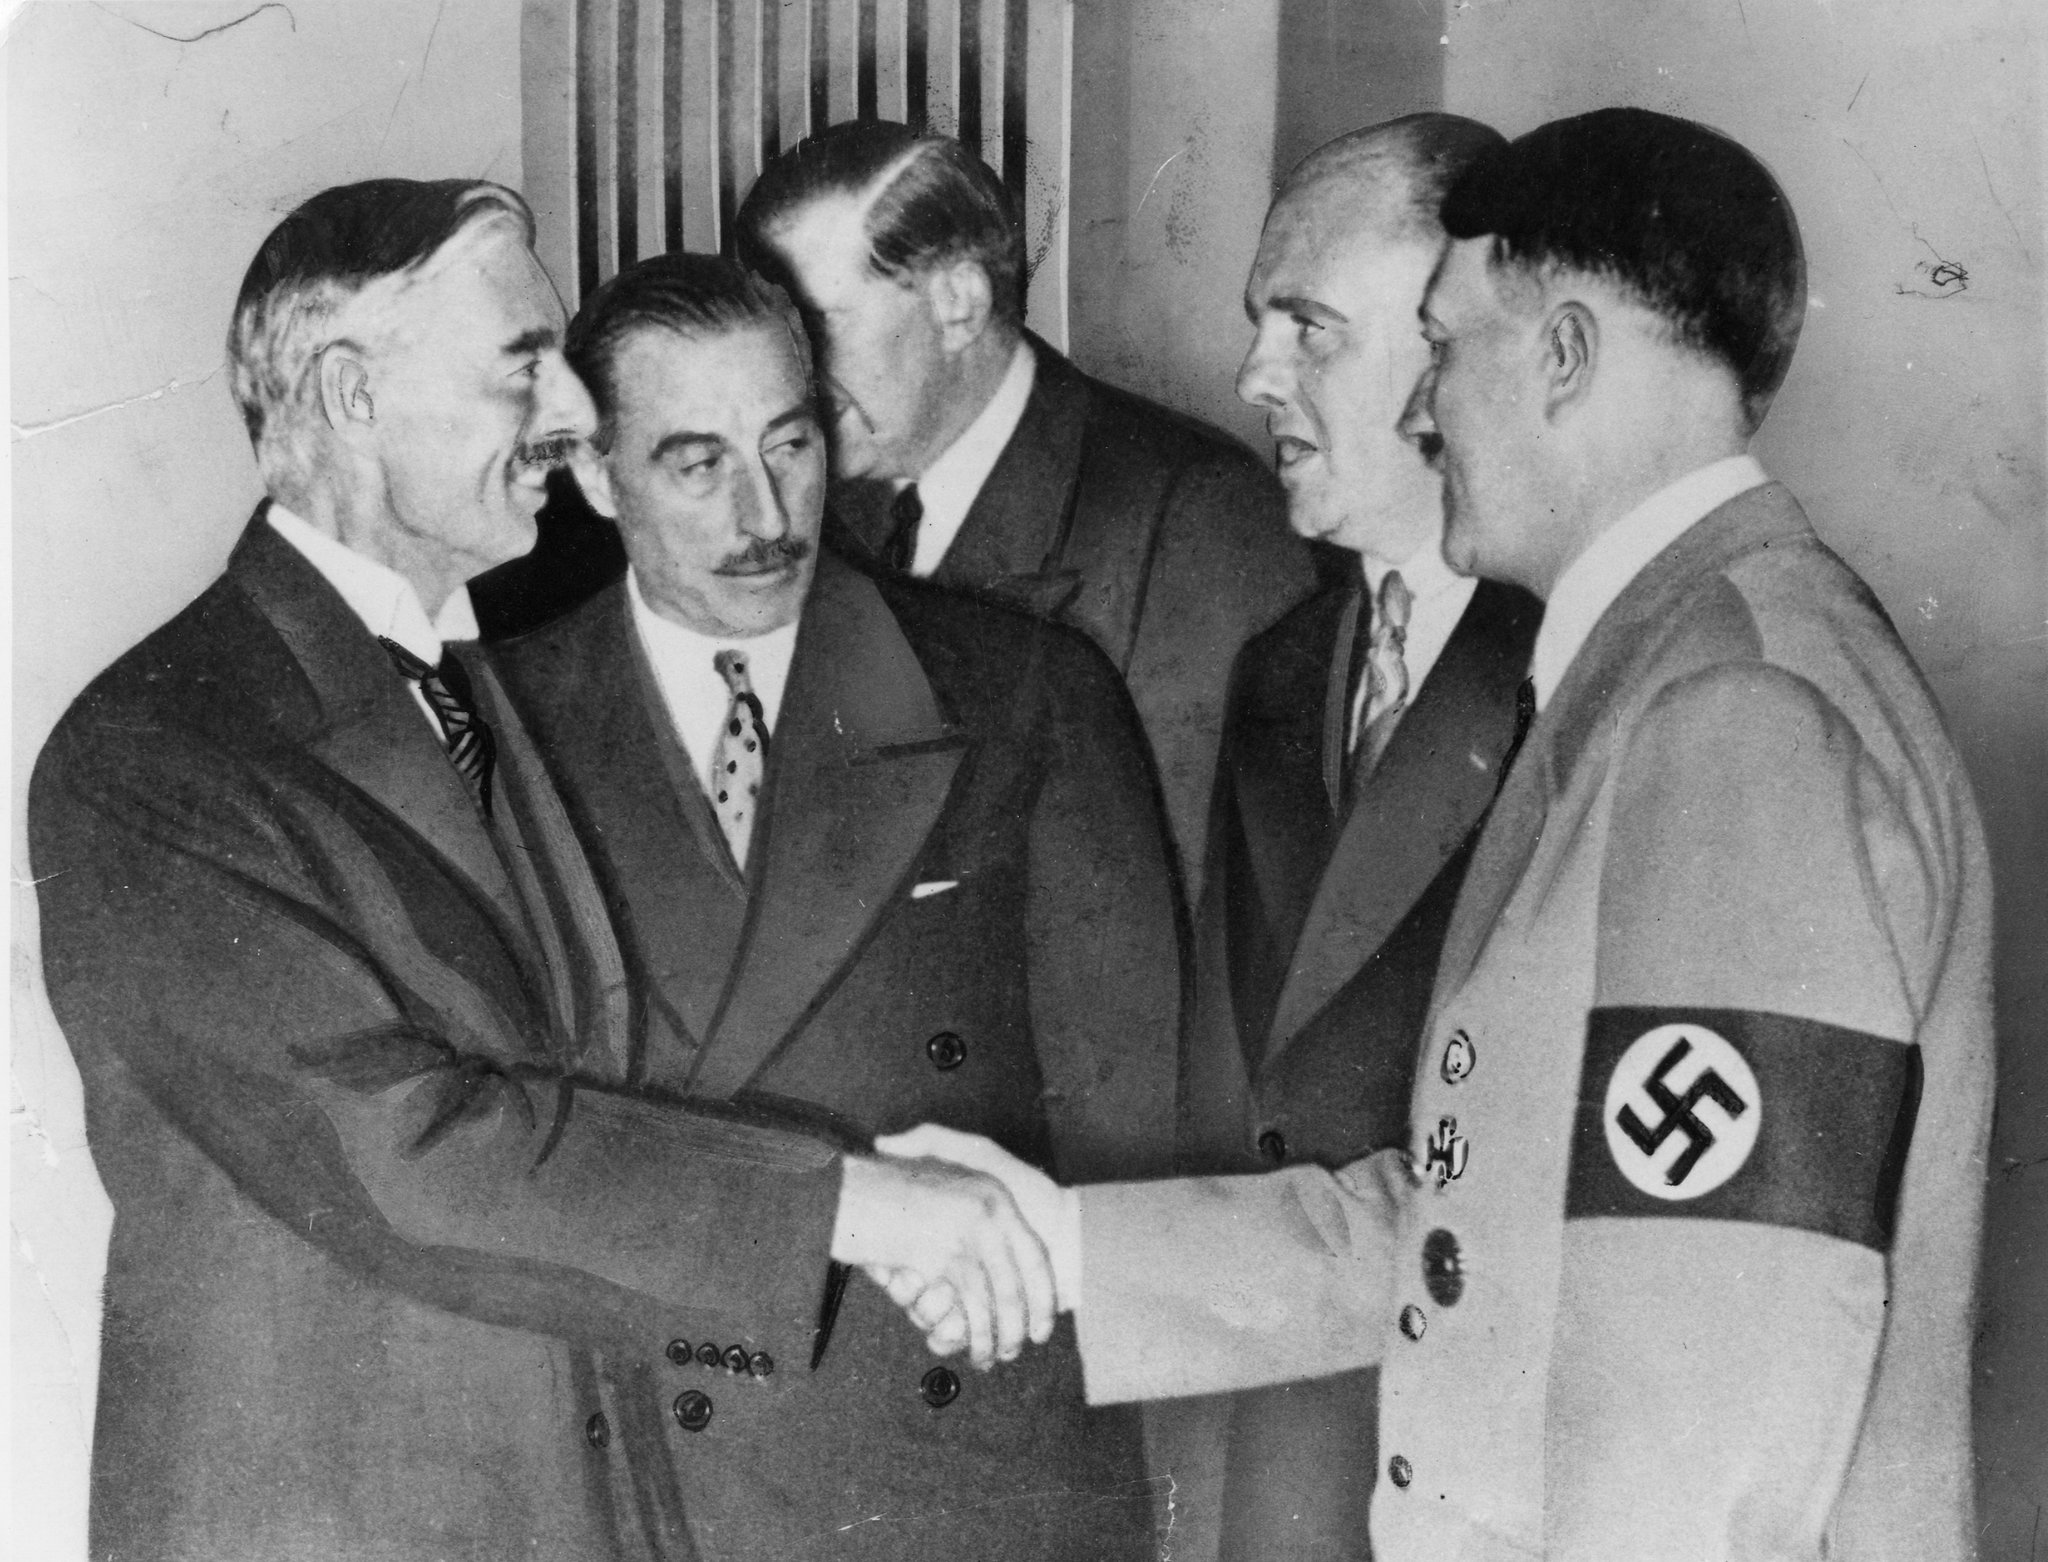
\includegraphics[width=\textwidth,height=.9\textheight,keepaspectratio]{Hitler appeasement.jpg}
\end{frame}

\begin{frame}{\LARGE Puzzle: Risk of Nuclear War}
    \centering
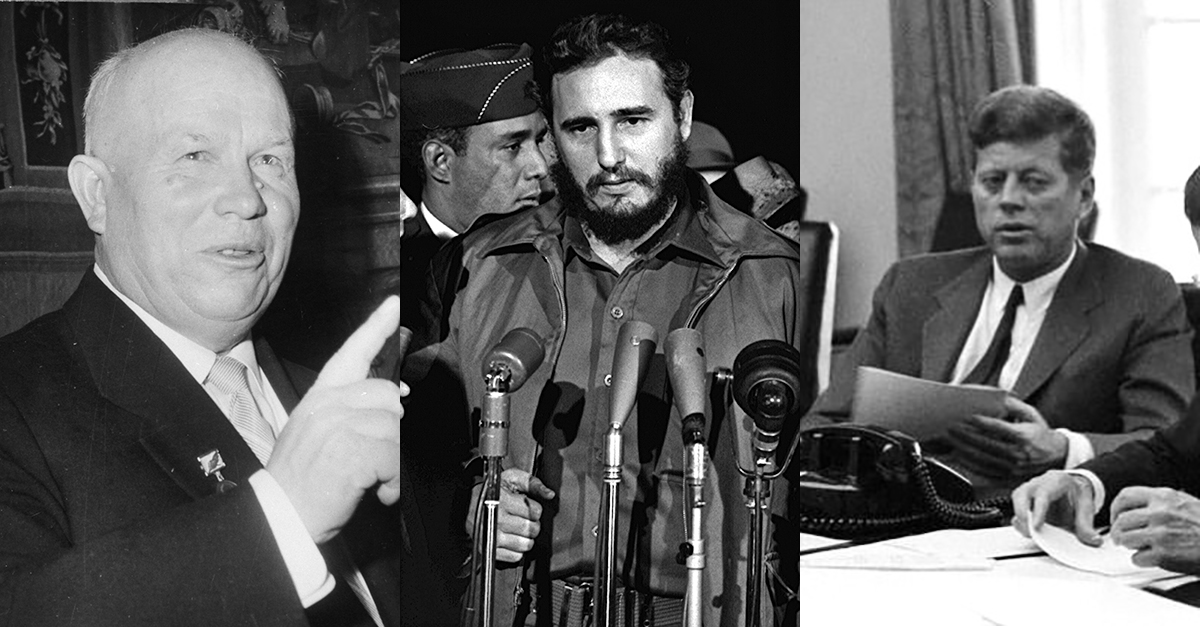
\includegraphics[width=\textwidth,height=0.8\textheight,keepaspectratio]{cuban missile crisis.jpg}
\end{frame}


\begin{frame}{\LARGE How do we study IR?}
\begin{itemize}
    \item We look at events, historical and current, and find something \textbf{puzzling} about them --- a phenomenon that needs to be explained. 
    \item We think \textbf{theoretically} about these phenomena --- we form models of human decision-making that can help us understand and explain puzzling behavior. \pause
    \item We test our theory using available information to find \textbf{generalizable explanations} --- using evidence from case studies, cross-national data, experiments. \pause
    \item Ultimately, by providing clear explanations of cause, we hope to both explain phenomena and/or provide guidance to policymakers. \pause
    \item That being said, our explanations are still \textbf{probabilistic}.
    \end{itemize}
\end{frame}



\end{document}
